\newpage
\section*{Bijlagen}
\addcontentsline{toc}{chapter}{Bijlagen}

\stepcounter{bijlage}
\subsection*{\hypertarget{bij:treasury}{Bijlage \thebijlage}: \gls{treasury} in kaart gebracht}
\addcontentsline{toc}{section}{Bijlage \thebijlage: treasury in kaart gebracht}
\begin{figure}[!hb]
    \centering
    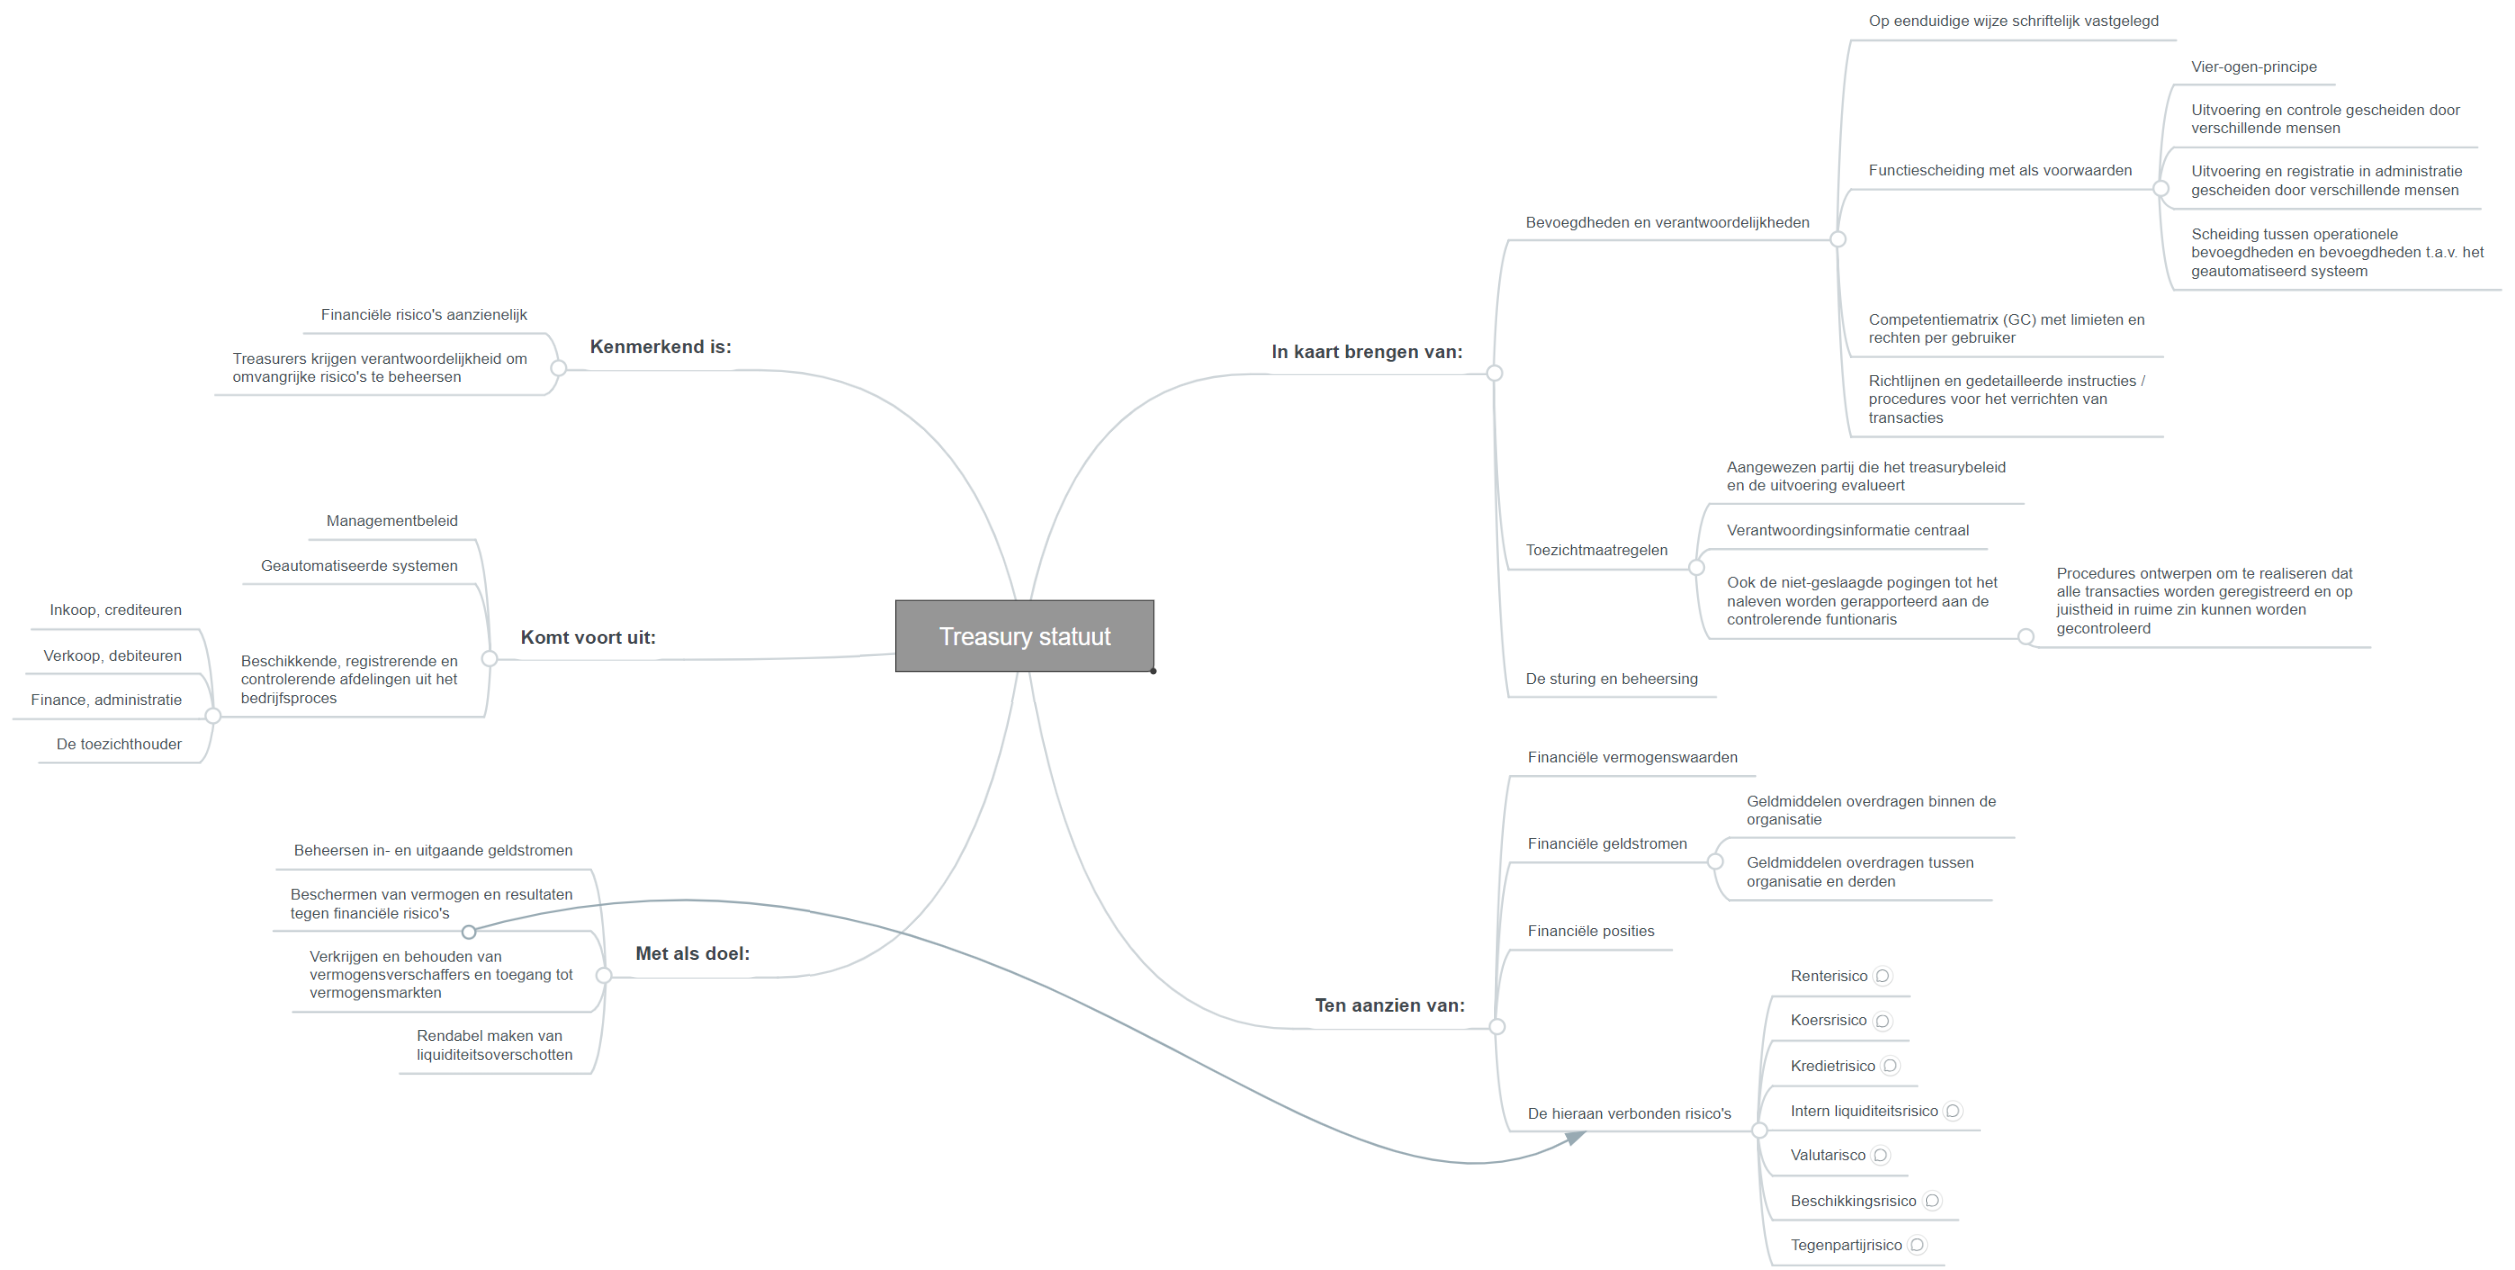
\includegraphics[angle=90,width=0.795\textwidth]{treasury}
    \label{fig:mmtreasury}
\end{figure}

\newpage
\stepcounter{bijlage}
\subsection*{\hypertarget{bij:inkoopproces}{Bijlage \thebijlage}: het inkoopproces (onder voorbehoud)}
\addcontentsline{toc}{section}{Bijlage \thebijlage: het inkoopproces (onder voorbehoud)}
\begin{figure}[!ht]
    \centering
    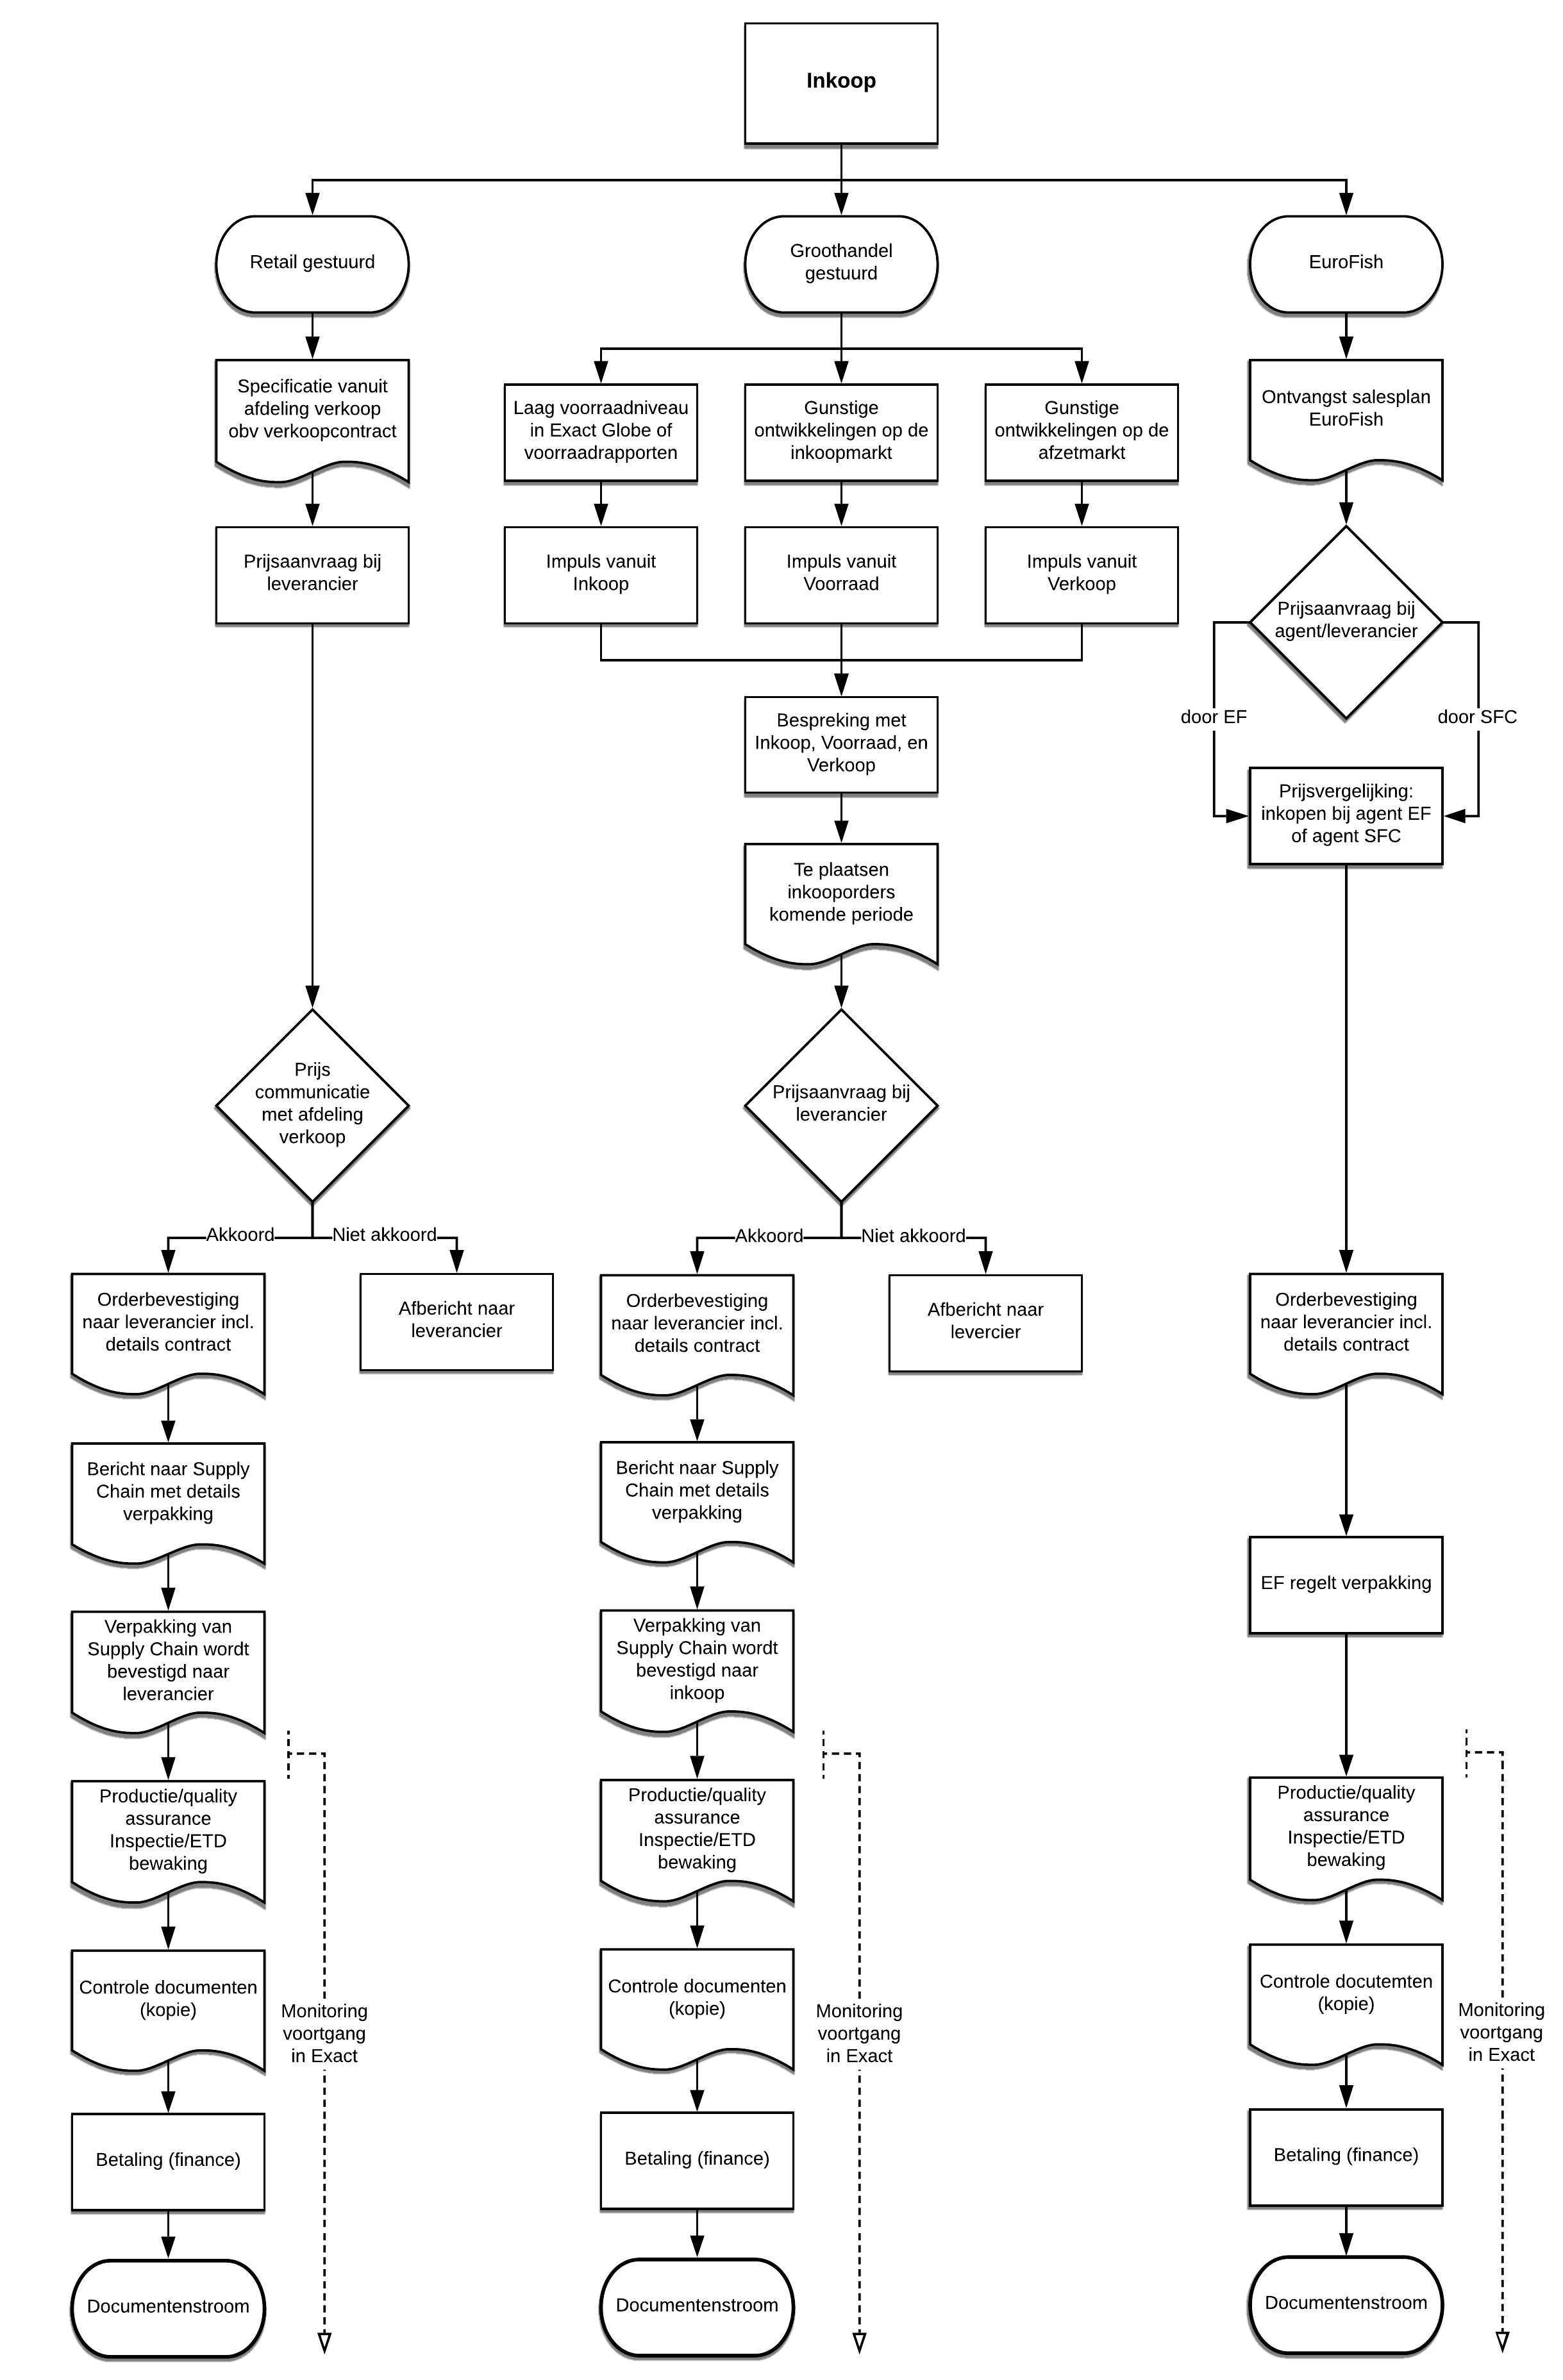
\includegraphics[width=1\textwidth]{inkoopproces}
    \label{fig:inkoopproces}
\end{figure}

\newpage
\stepcounter{bijlage}
\subsection*{\hypertarget{bij:treasury}{Bijlage \thebijlage}: de \gls{treasuryletter}}
\addcontentsline{toc}{section}{Bijlage \thebijlage: de treasury letter}
Zie ommezijde. {\color{red}Alleen de eerste twee pagina's nu.}

\includepdf[pages={1-2}]{../Bronnen/treasury.pdf}

\newpage
\stepcounter{bijlage}
\subsection*{\hypertarget{bij:aoib}{Bijlage \thebijlage}: AOIB beschrijving Seafood Connection}
\addcontentsline{toc}{section}{Bijlage \thebijlage: AOIB beschrijving Seafood Connection}
Zie ommezijde. {\color{red}Alleen de eerste twee pagina's nu.}

\includepdf[pages={1-2}]{../Bronnen/aoib.pdf}